% questions.tex —— 2011 年·浙江卷·文科 · 题目内容片段（无答案）
% 由 tools/generate_projects.py 依来源总账自 2011/2011_数学真题_浙江文_试题.md 生成，勿手改（改源 MD 后重跑）

\gkpart{一、选择题}

\begin{question}
\gkti{1}若 $P=\{x\mid x<1\}$，$Q=\{x\mid x>-1\}$，则\mbox{（　　）}

（A）$P\subseteq Q$

（B）$Q\subseteq P$

（C）$\complement_{\mathbf R}P\subseteq Q$

（D）$Q\subseteq\complement_{\mathbf R}P$

\end{question}
\begin{question}
\gkti{2}若复数 $z=1+\mathrm i$，$\mathrm i$ 为虚数单位，则 $(1+z)\cdot\bar z=$\mbox{（　　）}

（A）$1+3\mathrm i$

（B）$3+3\mathrm i$

（C）$3-\mathrm i$

（D）$3$

\end{question}
\begin{question}
\gkti{3}若实数 $x$，$y$ 满足不等式组 $\begin{cases}x+2y-5\geqslant0,\\2x+y-7\geqslant0,\\x\geqslant0,\ y\geqslant0,\end{cases}$ 则 $3x+4y$ 的最小值是\mbox{（　　）}

（A）$13$

（B）$15$

（C）$20$

（D）$28$

\end{question}
\begin{question}
\gkti{4}若直线 $l$ 不平行于平面 $\alpha$，且 $l\not\subset\alpha$，则\mbox{（　　）}

（A）$\alpha$ 内的所有直线与 $l$ 异面

（B）$\alpha$ 内不存在与 $l$ 平行的直线

（C）$\alpha$ 内存在唯一的直线与 $l$ 平行

（D）$\alpha$ 内的直线与 $l$ 都相交

\end{question}
\begin{question}
\gkti{5}在 $\triangle ABC$ 中，角 $A$，$B$，$C$ 所对的边分别为 $a$，$b$，$c$。若 $a\cos A=b\sin B$，则 $\sin A\cos A+\cos^2B=$\mbox{（　　）}

（A）$-\frac12$

（B）$\frac12$

（C）$-1$

（D）$1$

\end{question}
\begin{question}
\gkti{6}若 $a$，$b$ 为实数，则“$0<ab<1$”是“$b<\dfrac1a$”的\mbox{（　　）}

（A）充分而不必要条件

（B）必要而不充分条件

（C）充分必要条件

（D）既不充分也不必要条件

\Needspace{0.4\textheight}
\end{question}
\begin{question}
\gkti{7}若某几何体的三视图如图所示，则这个几何体的直观图可以是\mbox{（　　）}

（A）图 A

（B）图 B

（C）图 C

（D）图 D
\nopagebreak[4]
\begin{center}% 2011 年浙江卷文科第 7 题：三视图与四个直观图选项。
% 来源 PDF：普通高考/2011/2011浙江文.pdf，SHA-256 36931500dfd850579d93f0a685f0ccea25065c84c09db5157c451093d53b56f0。
% 原页：第 1 页第 1 栏，书页码 711。示意图。
\begin{tikzpicture}[>=stealth, semithick, font=\small, scale=0.85]
  \draw[thick] (0,0) rectangle (1.6,1.6);
  \draw[thick] (0,0.8)--(1.6,0.8);
  \node[below] at (0.8,-0.1) {正视图};
  \draw[thick] (2.4,0)--(2.4,1.6)--(3.3,1.6)--(3.8,0.9)--(3.8,0)--cycle;
  \node[below] at (3.1,-0.1) {侧视图};
  \draw[thick] (0.2,-2.4) rectangle (1.8,-0.8);
  \draw[thick] (0.2,-1.6)--(1.8,-1.6);
  \node[below] at (1.0,-2.5) {俯视图};
  % 选项
  \begin{scope}[xshift=4.2cm, yshift=-2.4cm, scale=0.5]
    \draw[thick] (0,0)--(2,0)--(2,1.2)--(0,1.2)--cycle;
    \draw[thick] (0,1.2)--(0.5,2.4)--(2.6,1.5)--(2,1.2);
    \draw[thick] (2,0)--(2.6,0.3)--(2.6,1.5);
    \node[below] at (1,-0.4) {(A)};
  \end{scope}
  \begin{scope}[xshift=7.4cm, yshift=-2.4cm, scale=0.5]
    \draw[thick] (0,0)--(2,0)--(2,1.2)--(0,1.2)--cycle;
    \draw[thick] (0,1.2)--(2,2.0)--(2.6,1.5)--(2,1.2);
    \draw[thick] (2,0)--(2.6,0.3)--(2.6,1.5);
    \node[below] at (1,-0.4) {(B)};
  \end{scope}
  \begin{scope}[xshift=10.6cm, yshift=-2.4cm, scale=0.5]
    \draw[thick] (0,0)--(2,0)--(2,1.2)--(0,1.2)--cycle;
    \draw[thick] (0.2,1.2)--(1.0,2.4)--(1.8,1.2);
    \draw[thick] (2,0)--(2.6,0.3)--(2.6,1.5)--(2,1.2);
    \node[below] at (1,-0.4) {(C)};
  \end{scope}
  \begin{scope}[xshift=13.8cm, yshift=-2.4cm, scale=0.5]
    \draw[thick] (0,0)--(2,0)--(2,1.2)--(0,1.2)--cycle;
    \draw[thick] (0,1.2)--(2,1.2)--(2,2.0)--(0,2.0)--cycle;
    \draw[thick] (2,0)--(2.6,0.3)--(2.6,2.3)--(2,2.0);
    \draw[thick] (0,2.0)--(0.6,2.3)--(2.6,2.3);
    \node[below] at (1,-0.4) {(D)};
  \end{scope}
\end{tikzpicture}
\end{center}
\nopagebreak[4]
\end{question}
\begin{question}
\gkti{8}从装有 $3$ 个红球、$2$ 个白球的袋中任取 $3$ 个球，则所取的 $3$ 个球中至少有 $1$ 个白球的概率是\mbox{（　　）}

（A）$\frac1{10}$

（B）$\frac3{10}$

（C）$\frac35$

（D）$\frac9{10}$

\end{question}
\begin{question}
\gkti{9}已知椭圆 $C_1:\dfrac{x^2}{a^2}+\dfrac{y^2}{b^2}=1$（$a>b>0$）与双曲线 $C_2:x^2-\dfrac{y^2}4=1$ 有公共的焦点，$C_2$ 的一条渐近线与以 $C_1$ 的长轴为直径的圆相交于 $A$，$B$ 两点。若 $C_1$ 恰好将线段 $AB$ 三等分，则\mbox{（　　）}

（A）$a^2=\frac{13}2$

（B）$a^2=13$

（C）$b^2=\frac12$

（D）$b^2=2$

\Needspace{0.4\textheight}
\end{question}
\begin{question}
\gkti{10}设函数 $f(x)=ax^2+bx+c$（$a$，$b$，$c\in\mathbf R$）。若 $x=-1$ 为函数 $y=f(x)\mathrm e^x$ 的一个极值点，则下列图象不可能为 $y=f(x)$ 图象的是\mbox{（　　）}

（A）图 A

（B）图 B

（C）图 C

（D）图 D
\nopagebreak[4]
\begin{center}% 2011 年浙江卷文科第 10 题：四个 y=f(x) 图象选项。
% 来源 PDF：普通高考/2011/2011浙江文.pdf，SHA-256 36931500dfd850579d93f0a685f0ccea25065c84c09db5157c451093d53b56f0。
% 原页：第 1 页第 2 栏，书页码 711。示意图；x=-1 用虚线标出。
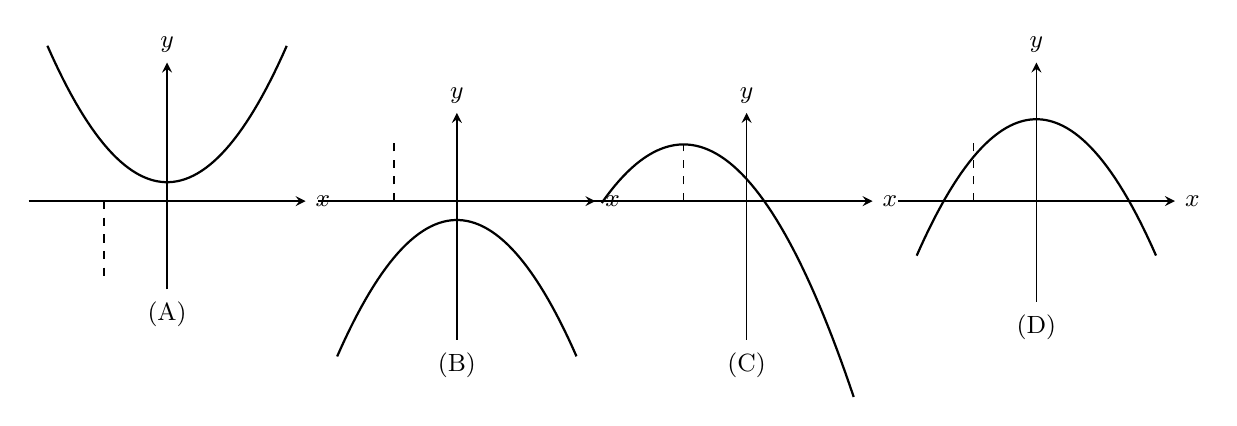
\begin{tikzpicture}[>=stealth, semithick, font=\small, scale=0.8]
  % (A) 开口向上，截距正
  \begin{scope}
    \draw[->] (-2.2,0)--(2.2,0) node[right] {$x$};
    \draw[->] (0,-1.4)--(0,2.2) node[above] {$y$};
    \draw[dashed] (-1,0)--(-1,-1.2);
    \draw[thick, domain=-1.9:1.9, samples=60] plot (\x,{0.6*\x*\x+0.3});
    \node at (0,-1.8) {(A)};
  \end{scope}
  % (B) 开口向下，截距负
  \begin{scope}[xshift=4.6cm]
    \draw[->] (-2.2,0)--(2.2,0) node[right] {$x$};
    \draw[->] (0,-2.2)--(0,1.4) node[above] {$y$};
    \draw[dashed] (-1,0)--(-1,1.0);
    \draw[thick, domain=-1.9:1.9, samples=60] plot (\x,{-0.6*\x*\x-0.3});
    \node at (0,-2.6) {(B)};
  \end{scope}
  % (C) 开口向下，顶点在 x=-1 附近，截距负
  \begin{scope}[xshift=9.2cm]
    \draw[->] (-2.6,0)--(2.0,0) node[right] {$x$};
    \draw[->] (0,-2.2)--(0,1.4) node[above] {$y$};
    \draw[dashed] (-1,0)--(-1,0.9);
    \draw[thick, domain=-2.3:1.7, samples=60] plot (\x,{-0.55*(\x+1)*(\x+1)+0.9});
    \node at (0,-2.6) {(C)};
  \end{scope}
  % (D) 开口向下，但截距为正（不可能）
  \begin{scope}[xshift=13.8cm]
    \draw[->] (-2.2,0)--(2.2,0) node[right] {$x$};
    \draw[->] (0,-1.6)--(0,2.2) node[above] {$y$};
    \draw[dashed] (-1,0)--(-1,1.0);
    \draw[thick, domain=-1.9:1.9, samples=60] plot (\x,{-0.6*\x*\x+1.3});
    \node at (0,-2.0) {(D)};
  \end{scope}
\end{tikzpicture}
\end{center}
\nopagebreak[4]
\end{question}
\gkpart{二、填空题}

\begin{question}
\gkti{11}设函数 $f(x)=\dfrac4{1-x}$。若 $f(a)=2$，则实数 $a=$ $\underline{\qquad}$。

\end{question}
\begin{question}
\gkti{12}若直线 $x-2y+5=0$ 与直线 $2x+my-6=0$ 互相垂直，则实数 $m=$ $\underline{\qquad}$。

\Needspace{0.4\textheight}
\end{question}
\begin{question}
\gkti{13}某小学为了解学生数学课程的学习情况，在 $3000$ 名学生中随机抽取 $200$ 名，并统计这 $200$ 名学生的某次数学考试成绩，得到了样本的频率分布直方图（如图）。根据频率分布直方图，$3000$ 名学生在该次数学考试中成绩小于 $60$ 分的学生数是 $\underline{\qquad}$。
\nopagebreak[4]
\begin{center}% 2011 年浙江卷文科第 13 题：样本频率分布直方图。
% 来源 PDF：普通高考/2011/2011浙江文.pdf，SHA-256 36931500dfd850579d93f0a685f0ccea25065c84c09db5157c451093d53b56f0。
% 原页：第 1 页第 2 栏下部，书页码 711。组距 10；<60 分组高为 0.002,0.006,0.012。
\begin{tikzpicture}[>=stealth, semithick, font=\small, x=0.9cm, y=22cm]
  \draw[->] (0,0)--(10,0) node[right] {成绩/分};
  \draw[->] (0,0)--(0,0.032) node[above] {$\dfrac{\text{频率}}{\text{组距}}$};
  \foreach \x/\h in {3/0.002,4/0.006,5/0.012,6/0.024,7/0.028}{
    \draw (\x-0.5,0) rectangle (\x+0.5,\h);
  }
  \foreach \x in {3,4,5,6,7} \node[below] at (\x,0) {$\x0$};
  \foreach \y in {0.002,0.006,0.012,0.024,0.028} \node[left] at (0,\y) {\y};
  \node[below left] at (0,0) {$O$};
\end{tikzpicture}
\end{center}
\nopagebreak[4]
\Needspace{0.4\textheight}
\end{question}
\begin{question}
\gkti{14}某程序框图如图所示，则该程序运行后输出的 $k$ 的值是 $\underline{\qquad}$。
\nopagebreak[4]
\begin{center}% 2011 年浙江卷理科第 12 题：程序框图。
% 来源 PDF：普通高考/2011/2011浙江理.pdf，SHA-256 0239778f574bc3ce6d7aca5024aa6333f80d131abaf699f79c46472394f8cd65。
% 原页：第 1 页第 2 栏中部，书页码 709。
\begin{tikzpicture}[>=stealth, semithick, font=\small]
  \node[draw, rounded corners=0.12cm, minimum width=1.2cm, minimum height=0.5cm] (start) at (0,0) {开始};
  \node[draw, minimum width=1.4cm, minimum height=0.5cm] (k2) at (0,-1.1) {$k=2$};
  \node[draw, minimum width=1.8cm, minimum height=0.5cm] (inc) at (0,-2.2) {$k=k+1$};
  \node[draw, minimum width=1.8cm, minimum height=0.5cm] (a) at (0,-3.3) {$a=4^k$};
  \node[draw, minimum width=1.8cm, minimum height=0.5cm] (b) at (0,-4.4) {$b=k^4$};
  \node[draw, diamond, aspect=1.7, minimum width=1.6cm, minimum height=0.9cm] (test) at (0,-5.8) {$a>b$};
  \node[draw, trapezium, trapezium left angle=72, trapezium right angle=108,
        minimum width=1.6cm, minimum height=0.55cm] (out) at (0,-7.2) {输出 $k$};
  \node[draw, rounded corners=0.12cm, minimum width=1.2cm, minimum height=0.5cm] (stop) at (0,-8.4) {结束};
  \draw[->] (start.south)--(k2.north);
  \draw[->] (k2.south)--(inc.north);
  \draw[->] (inc.south)--(a.north);
  \draw[->] (a.south)--(b.north);
  \draw[->] (b.south)--(test.north);
  \draw[->] (test.south)--(out.north) node[midway, right] {是};
  \draw[->] (out.south)--(stop.north);
  \draw[->] (test.east) -- ++(1.4,0) |- (inc.east) node[pos=0.25, right] {否};
\end{tikzpicture}
\end{center}
\nopagebreak[4]
\end{question}
\begin{question}
\gkti{15}若平面向量 $\boldsymbol\alpha$、$\boldsymbol\beta$ 满足 $|\boldsymbol\alpha|=1$，$|\boldsymbol\beta|\leqslant1$，且以向量 $\boldsymbol\alpha$、$\boldsymbol\beta$ 为邻边的平行四边形的面积为 $\dfrac12$，则 $\boldsymbol\alpha$ 和 $\boldsymbol\beta$ 的夹角 $\theta$ 的取值范围是 $\underline{\qquad}$。

\end{question}
\begin{question}
\gkti{16}若实数 $x$，$y$ 满足 $x^2+y^2+xy=1$，则 $x+y$ 的最大值是 $\underline{\qquad}$。

\end{question}
\begin{question}
\gkti{17}若数列 $\left\{n(n+4)\left(\dfrac23\right)^n\right\}$ 中的最大项是第 $k$ 项，则 $k=$ $\underline{\qquad}$。

\end{question}
\gkpart{三、解答题}

\Needspace{0.4\textheight}
\begin{question}
\gkti{18}已知函数 $f(x)=A\sin\left(\dfrac\pi3x+\varphi\right)$，$x\in\mathbf R$，$A>0$，$0<\varphi<\dfrac\pi2$。$y=f(x)$ 的部分图象如图所示，$P$，$Q$ 分别为该图象的最高点和最低点，点 $P$ 的坐标为 $(1,A)$。

（1） 求 $f(x)$ 的最小正周期及 $\varphi$ 的值；

（2） 若点 $R$ 的坐标为 $(1,0)$，$\angle PRQ=\dfrac{2\pi}3$，求 $A$ 的值。
\nopagebreak[4]
\begin{center}% 2011 年浙江卷文科第 18 题：f(x)=A sin(πx/3+φ) 的部分图象。
% 来源 PDF：普通高考/2011/2011浙江文.pdf，SHA-256 36931500dfd850579d93f0a685f0ccea25065c84c09db5157c451093d53b56f0。
% 原页：第 1 页第 3 栏，书页码 711。P(1,A) 最高点，Q(4,-A) 最低点，R(1,0)。
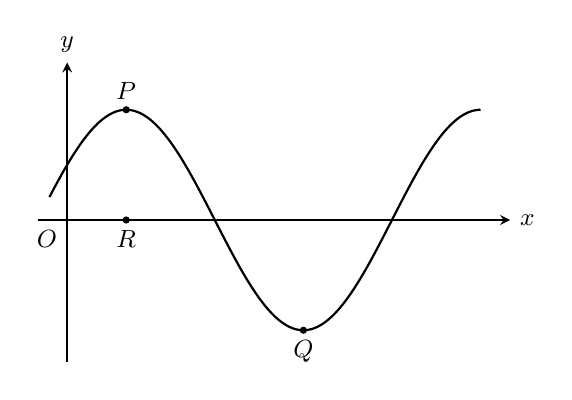
\begin{tikzpicture}[>=stealth, semithick, font=\small, x=0.75cm, y=1.0cm]
  \draw[->] (-0.5,0)--(7.5,0) node[right] {$x$};
  \draw[->] (0,-1.8)--(0,2.0) node[above] {$y$};
  \node[below left] at (0,0) {$O$};
  \draw[thick, domain=-0.3:7.0, samples=200] plot (\x,{1.4*sin(deg(pi*\x/3+pi/6))});
  \fill (1,1.4) circle (1.3pt) node[above] {$P$};
  \fill (4,-1.4) circle (1.3pt) node[below] {$Q$};
  \fill (1,0) circle (1.3pt) node[below] {$R$};
\end{tikzpicture}
\end{center}
\nopagebreak[4]
\end{question}
\begin{question}
\gkti{19}已知公差不为 $0$ 的等差数列 $\{a_n\}$ 的首项 $a_1$ 为 $a$（$a\in\mathbf R$），且 $\dfrac1{a_1}$，$\dfrac1{a_2}$，$\dfrac1{a_4}$ 成等比数列。

（1） 求数列 $\{a_n\}$ 的通项公式；

（2） 对 $n\in\mathbf N^*$，试比较 $\dfrac1{a_2}+\dfrac1{a_{2^2}}+\dfrac1{a_{2^3}}+\cdots+\dfrac1{a_{2^n}}$ 与 $\dfrac1{a_1}$ 的大小。

\Needspace{0.4\textheight}
\end{question}
\begin{question}
\gkti{20}如图，在三棱锥 $P-ABC$ 中，$AB=AC$，$D$ 为 $BC$ 的中点，$PO\perp$ 平面 $ABC$，垂足 $O$ 落在线段 $AD$ 上。

（1） 证明：$AP\perp BC$；

（2） 已知 $BC=8$，$PO=4$，$AO=3$，$OD=2$，求二面角 $B-AP-C$ 的大小。
\nopagebreak[4]
\begin{center}% 2011 年浙江卷理科第 20 题：三棱锥 P-ABC，O 在 AD 上，PO⊥平面 ABC。
% 来源 PDF：普通高考/2011/2011浙江理.pdf，SHA-256 0239778f574bc3ce6d7aca5024aa6333f80d131abaf699f79c46472394f8cd65。
% 原页：第 2 页第 1 栏，书页码 710。示意。
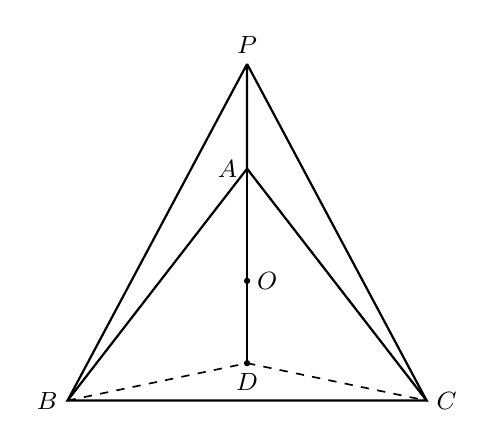
\begin{tikzpicture}[>=stealth, semithick, font=\small, scale=0.95]
  \coordinate (D) at (0,0);
  \coordinate (B) at (-2.4,-0.5);
  \coordinate (C) at (2.4,-0.5);
  \coordinate (A) at (0,2.6);
  \coordinate (O) at (0,1.1);
  \coordinate (P) at (0,4.0);
  \draw[thick] (A)--(B)--(C)--cycle;
  \draw[thick] (P)--(A) (P)--(B) (P)--(C);
  \draw[dashed] (A)--(C);
  \draw[dashed] (P)--(O);
  \draw[dashed] (B)--(D);
  \draw[dashed] (D)--(C);
  \draw (A)--(D);
  \fill (D) circle (1.2pt) node[below] {$D$};
  \fill (O) circle (1.2pt) node[right] {$O$};
  \node[left] at (A) {$A$};
  \node[left] at (B) {$B$};
  \node[right] at (C) {$C$};
  \node[above] at (P) {$P$};
\end{tikzpicture}
\end{center}
\nopagebreak[4]
\end{question}
\begin{question}
\gkti{21}设函数 $f(x)=a^2\ln x-x^2+ax$，$a>0$。

（1） 求 $f(x)$ 的单调区间；

（2） 求所有实数 $a$，使 $\mathrm e-1\leqslant f(x)\leqslant\mathrm e^2$ 对 $x\in[1,\mathrm e]$ 恒成立。

注：$\mathrm e$ 为自然对数的底数。

\Needspace{0.4\textheight}
\end{question}
\begin{question}
\gkti{22}如图，设 $P$ 为抛物线 $C_1:x^2=y$ 上的动点，过点 $P$ 作圆 $C_2:x^2+(y+3)^2=1$ 的两条切线，交直线 $l:y=-3$ 于 $A$，$B$ 两点。

（1） 求 $C_2$ 的圆心 $M$ 到抛物线 $C_1$ 准线的距离。

（2） 是否存在点 $P$，使线段 $AB$ 被抛物线 $C_1$ 在点 $P$ 处的切线平分？若存在，求出点 $P$ 的坐标；若不存在，请说明理由。
\nopagebreak[4]
\begin{center}% 2011 年浙江卷文科第 22 题：抛物线 x^2=y、圆 x^2+(y+3)^2=1、直线 y=-3。
% 来源 PDF：普通高考/2011/2011浙江文.pdf，SHA-256 36931500dfd850579d93f0a685f0ccea25065c84c09db5157c451093d53b56f0。
% 原页：第 2 页第 3 栏，书页码 712。示意图。
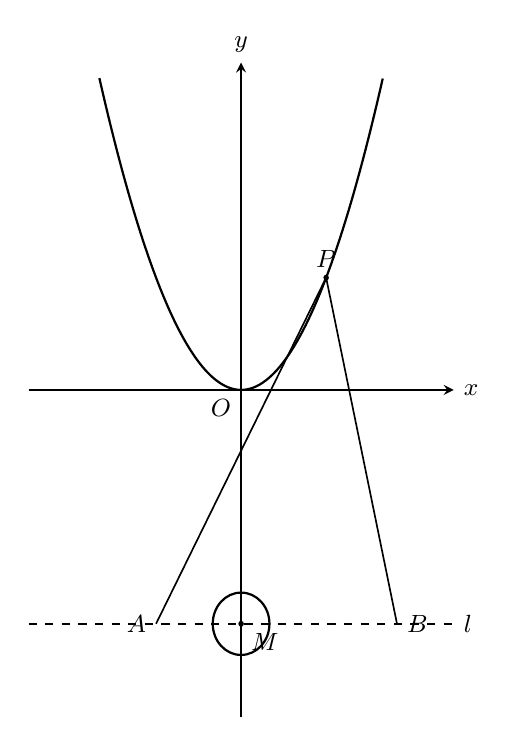
\begin{tikzpicture}[>=stealth, semithick, font=\small, scale=0.9, yscale=1.1]
  \draw[->] (-3,0)--(3,0) node[right] {$x$};
  \draw[->] (0,-4.2)--(0,4.2) node[above] {$y$};
  \draw[thick, domain=-2:2, samples=100] plot (\x,{\x*\x});
  \draw[thick] (0,-3) circle (0.4);
  \fill (0,-3) circle (1.1pt) node[below right] {$M$};
  \draw[dashed] (-3,-3)--(3,-3) node[right] {$l$};
  \coordinate (P) at (1.2,1.44);
  \fill (P) circle (1.1pt) node[above] {$P$};
  \draw (P)--(-1.2,-3) node[left] {$A$};
  \draw (P)--(2.2,-3) node[right] {$B$};
  \node[below left] at (0,0) {$O$};
\end{tikzpicture}
\end{center}
\nopagebreak[4]

\end{question}